\documentclass{beamer}
\usetheme{metropolis}

\usefonttheme{serif} % default family is serif

\setbeamertemplate{section in toc}[sections numbered]
\setbeamertemplate{subsection in toc}[subsections numbered]

\title{Macroeconomics 2 Presentation}
\subtitle{Article review :\\ Gabaix, Xavier. 2020. "A Behavioral New Keynesian Model." American Economic Review, 110(8): 2271-2327}
\author{GUGELMO CAVALHEIRO DIAS Paulo \\ MITASH Nayanika \\ WANG Shang}
\institute{Sciences Po}
\date{\today}


\newcommand\ReduceFont{\fontsize{10}{7.2}\selectfont}

\begin{document}

\begin{frame}
    \titlepage
\end{frame}

\begin{frame}
    \ReduceFont
    \frametitle{Outline}
    \tableofcontents[hideallsubsections]
\end{frame}

\section{Contextualization}
\begin{frame}
    \tableofcontents[currentsection, hideothersubsections, sections=\value{section}]
\end{frame}

\subsection{Goal of the paper}
\begin{frame}{\subsecname}
    Content of the Goal of the paper.
\end{frame}

\subsection{Literature of the topic}
\begin{frame}
    Content of the the Literature.
\end{frame}

\section{Baseline model of the paper}
\begin{frame}
    \ReduceFont
    \tableofcontents[currentsection, hideallsubsections]
\end{frame}

\begin{frame}
    \tableofcontents[currentsection, hideothersubsections, sections=\value{section}]
\end{frame}

\subsection{Household's Problem}

\subsubsection{Objective function}
\begin{frame}{\subsecname}
    \begin{equation}\tag{3}
        \label{3}
        U = \mathbb{E}\left[\sum_{t=0}^{\infty}\beta^{t}u(c_t,N_t)\right]
    \end{equation}
    With
    \begin{equation*}
    u(c_t,N_t) = \frac{c^{1-\gamma}-1}{1-\gamma}-\frac{N^{1+\phi}}{1+\phi}
    \end{equation*}
    So we have the following objective function of the household: 
    \begin{equation*}
        U = \mathbb{E}\left[\sum_{t=0}^{\infty}\beta^{t}\left(\frac{c^{1-\gamma}-1}{1-\gamma}-\frac{N^{1+\phi}}{1+\phi}\right)\right]
    \end{equation*}
    Subject to 
  \begin{equation}\tag{4}
        k_{t+1}=(1+r_t)(k_t-c_t+y_t)
    \end{equation} 
with $y_t=w_t\cdot N_{t}+y_{t}^{f}$ and $Y_{i t}=N_{i t} e^{\zeta_t}$ where $\zeta_t$ follows an AR(1) process with mean 0

Deterministic steady state $\bar{c}=\bar{N}=\bar{w}=\bar{y}=1$

    
    
\end{frame}

\subsubsection{State Vector}
\begin{frame}{\subsecname}
Law of motion of state vector
\begin{equation}\tag{5}
    \bm{X}_{t+1}=\bm{G}^{\bm{X}}\left(\bm{X}_{t},\bm{\epsilon}_{t+1}\right)
\end{equation}
Decomposing variables as deviations from steady-state
\begin{align*}
    r_{t} &= \bar{r} + \hat{r}_{t} & y_{t} &= \bar{y} + \hat{y}_{t}
\end{align*}
Where the deviations are functions of the State Vector
\begin{align*}
   \hat{r}_{t} &= \hat{r}(\bm{X}_t) & \hat{y}_{t} &= \hat{y}(N_{t},\bm{X}_{t}) := {w}(\bm{X}_{t})N_{t} + y^{f}(\bm{X}_t)- \bar{y}
\end{align*}
Private financial wealth
\begin{equation}\tag{6}
    k_{t+1}=G^{k}(c_{t},N_{t}, k_{t}, \bm{X}_t):= (1+\bar{r}+\hat{r}(\bm{X}_{t}))(k_{t}+\bar{y}+\hat{y}(N_{t},\bm{X}_t)-c_{t})
\end{equation}
\end{frame}

\subsubsection{Linearisation}
\begin{frame}{\subsecname}

Linearisation of the State vector
\begin{equation}\tag{7}
    \bm{X}_{t+1}=\bm{\Gamma}\bm{X}_{t}+\bm{\epsilon}_{t+1}
\end{equation} 
Linearisation of the deviations
\begin{equation*}
    \hat{r}(\bm{X})= \bm{b}_{\bm{X}}^{r} \bm{X}
\end{equation*}

\end{frame}

\subsubsection{Behavioural Model: Discounting of State Variable}
\begin{frame}{\subsecname}
Cognitive Discounting of the State vector (Non-Linearised and Linearised)


\begin{align}
\tag{8}
&\bm{X}_{t+1}=\bar{m}\cdot\bm{G}^{\bm{X}}(\bm{X}_{t},\bm{\epsilon}_{t+1}) \\
\tag{9}
&\bm{X}_{t+1}=\bar{m}(\bm{\Gamma}\bm{X}_{t}+\bm{\epsilon}_{t+1})
\end{align}

Subjective Expectation
\begin{align*}
\mathbb{E}_{t}^{BR}\left[\bm{X}_{t+1}\right]&= \bar{m}\bm{\Gamma}\bm{X_{t}}\\
\mathbb{E}_{t}^{BR}\left[\bm{X}_{t+k}\right]&=\bar{m}^{k}\bm{\Gamma}^{k}\bm{X_{t}}\\
\tag{10}\mathbb{E}_{t}^{BR}\left[\bm{X}_{t+k}\right]&=\bar{m}^{k}\mathbb{E}_{t}\left[\bm{X}_{t+k}\right]
\end{align*}
\end{frame}
\subsubsection{Behavioural Model: Discounting of All Variables}
\begin{frame}{\subsecname}
Cognitive discounting of all Variables (LEMMA 1)
\begin{equation}\tag{11}
    \mathbb{E}_{t}^{BR}\left[z\left(\bm{X}_{t+k}\right)\right]=\bar{m}^{k}\mathbb{E}_{t}\left[z\left(\bm{X}_{t+k}\right)\right]
\end{equation}
For Example
\begin{equation}\tag{12}
    \mathbb{E}_{t}^{BR}\left[\bar{r}+\hat{r}\left(\bm{X}_{t+k}\right)\right]=\bar{r}+\bar{m}^{k}\mathbb{E}_{t}\left[\hat{r}(\bm{X}_{t+k})\right]
\end{equation}

\end{frame}


\subsection{Firm's Problem}

\subsubsection{Firm's Problem}
\begin{frame}{\subsecname}
Firm's Aggregate Price Level

\begin{equation}\tag{13}
    P_{t}=\left(\int_{0}^{1}P_{it}^{1-\varepsilon}\,di\right)^{\frac{1}{1-\varepsilon}}
\end{equation}

Firm's Maximise their real profit
\begin{equation*}
    \nu_{\tau} = \left(\frac{P_{i\tau}}{P_{\tau}}-MC_{\tau}\right)\left(\frac{P_{i\tau}}{P_{\tau}}\right)^{-\varepsilon} c_{\tau}
\end{equation*}
Where
\begin{itemize}
\item    $\left(\frac{P_{i\tau}}{P_{\tau}}\right)^{-\varepsilon} c_{\tau}$ is the total demand for the firm's good 
\item $MC_{t}=(1-\tau_{f})(\omega_{t}/e^{\zeta{t}})=(1-\tau_{f})e^{-\mu_{t}}$ and $\mu_{t} :=\zeta_{t}- \ln \omega_{t}$ is the labour wedge and $\tau_{f}= 1/\varepsilon$ which corrects the price distortions
\end{itemize}
 
    

\end{frame}
\subsubsection{Firm's Real Profits}
\begin{frame}{\subsecname}
Firm's real profit
\begin{equation*}
    \nu_{\tau} = \left(\frac{P_{i\tau}}{P_{\tau}}-MC_{\tau}\right)\left(\frac{P_{i\tau}}{P_{\tau}}\right)^{-\varepsilon} c_{\tau}
\end{equation*}

\begin{equation}\tag{14}
    \nu^{0}(q_{i\tau},\mu_{\tau},c_{\tau}):=\left(e^{q_{i\tau}}-(1-\tau_{f})e^{-\mu_{\tau}}\right)e^{-\varepsilon q_{i\tau}}c_{\tau}
\end{equation} where 
\begin{itemize}
    \item  $q_{i\tau}=\ln\left(\frac{P_{i\tau}}{P_{\tau}}\right)= p_{i\tau}-p_{\tau}$ hence $\left(\frac{P_{i\tau}}{P_{\tau}}\right)= e^{q_{i\tau}}$
\end{itemize}


\end{frame}
\subsubsection{Firm's Real Profits}
\begin{frame}{\subsecname}

$\mathbf{X}_\tau=\left(\mathbf{X}_\tau^{\mathcal{M}}, \Pi_\tau\right)$ where $\Pi_\tau:= p_{\tau}-p_{t}$ and $\mathbf{X}_\tau^{\mathcal{M}}$ is vector including macroeconomic variables.

 If firm hasn't changed its price between $t$ and $\tau$
then its real price $q_{i\tau}= q_{it}- \Pi_{\tau}$ 

Hence the flow of profit 
\begin{equation}\tag{15}
    \nu\left(q_{it},\bm{X}{\tau}\right):=\nu^{0}\left(q_{it}-\Pi(\bm{X}{\tau}),\mu(\bm{X}{\tau}),c(\bm{X}_{\tau})\right)
\end{equation} 

\end{frame}
\subsubsection{Firm's Maximisation Problem}
\begin{frame}{\subsecname}
Maximisation problem for a Traditional Calvo Firm who can adjusts its prices
\begin{equation}\tag{16}
\max_{\text{q}_{it}} \mathbb{E}_{t} \sum_{\tau=t}^{\infty}(\beta\theta)^{\tau-t} \frac{c\left(\bm{X_{\tau}}\right)^{-\gamma}}{\left(\bm{X_{t}}\right)^{-\gamma}} \nu\left(q_{it},\bm{X}{\tau}\right)
\end{equation}
Behavioural Counterpart
\begin{equation}\tag{17}
    \max_{q_{it}}{\mathbb{E}_{t}^{BR} \left[\sum_{\tau=t}^{\infty}(\beta\theta)^{\tau-t}\frac{c\left(\bm{X}_{\tau}^{-\gamma}\right)}{c\left(\bm{X}_{t}^{-\gamma}\right)} \nu\left(q_{it,\bm{X}_{\tau}}\right) \right]}
\end{equation} 
\end{frame}
\subsection{Solution}

\subsubsection{Euler and Static FOC for Labour}
\begin{frame}{\subsecname}
Solving the Household's Maximisation Problem we get:

Euler
\begin{equation}\tag{18}
    \hat{c}_{t}=\mathbb{E}_{t}\left[\hat{c}_{t+1}-\frac{1}{\gamma R}\hat{r}_{t}\right]
\end{equation}

\begin{equation*}
    \hat{c}_{t}=\mathbb{E}_{t}\left[\hat{c}_{t+1}\right]-\sigma\hat{r}_{t}
\end{equation*}

Static First Order Condition for Labour Supply
\begin{equation}\tag{20}
    N^{\phi}_{t}=\omega_{t}c_{t}^{\gamma}
\end{equation}

\end{frame}

\subsubsection{Behavioural Equation}
\begin{frame}{\subsecname}

Using Lemma 1
\begin{equation*}
    \mathbb{E}_{t}^{BR}\left[z\left(\bm{X}_{t+k}\right)\right]=\bar{m}^{k}\mathbb{E}_{t}\left[z\left(\bm{X}_{t+k}\right)\right]
\end{equation*}
We get Behavioural Euler Equation
\begin{equation*}
    \hat{c}(\bm{X_{t}})=\mathbb{E}_{t}^{BR}\left[\hat{c}(\bm{X_{t+1}})\right]-\frac{1}{\gamma R}\hat{r}_{t}
\end{equation*}
\begin{equation}\tag{19}
    \hat{c}_{t}=M\cdot\mathbb{E}_{t}\left[\hat{c}_{t+1}\right]-\sigma\hat{r}_{t}
\end{equation} 
here $M=\bar{m}$
\end{frame}

\subsubsection{Natural Economy/Flexible Price Economy}
\begin{frame}{\subsecname}

Natural Rate Output without pricing frictions
\begin{equation}\tag{21}
    \hat{c}_{t}^{n}=\frac{1+\phi}{\gamma+\phi}\zeta_{t}
\end{equation}
\begin{equation}\tag{22}
    \hat{c}^{n}_{t} = M\cdot\mathbb{E}_{t}\left[\hat{c}^{n}_{t+1}\right]-\sigma\hat{r}^{n}_{t}
\end{equation}
Natural Interest Rate (here natural interest is the same as the pure natural interest rate where there are no budget deficits)
\begin{equation}\tag{23}
    r^{n0}_{t}=\bar{r}+\frac{1+\phi}{\sigma(\gamma+\phi)}\left(M\cdot\mathbb{E}_{t}\left[\zeta_{t+1}\right]-\zeta_{t}\right)
\end{equation}
\end{frame}

\subsubsection{Behavioural Discounted Euler}
\begin{frame}{\subsecname}
Behavioural Discounted Euler Equation
\begin{equation}\tag{24}
    x_{t}=M\cdot\mathbb{E}_{t}\left[x_{t+1}\right]-\sigma(\hat{r}_{t}-\hat{r}^{n}_{t})
\end{equation}
\begin{equation}\tag{25}
    x_{t}=M\cdot\mathbb{E}_{t}\left[x_{t+1}\right]-\sigma(i_{t}-\mathbb{E}_{t}\left[\pi_{t+1}\right]-r^{n}_{t})
\end{equation}
 where
\begin{itemize}
    \item $\hat r_{t}= r_{t}- \bar r = (i_{t}-\mathbb{E}_{t}\left[\pi_{t+1}\right]-\bar{r})$
    \item $\hat r_{t}^{n}= r_{t}^{n}- \bar r$ 
    \item Therefore $\hat{r_{t}}-\hat{r}^{n}_{t}=(i_{t}-\mathbb{E}_{t}\left[\pi_{t+1}\right]-\bar{r})$
\end{itemize}

Iterative Version of the Behavioural Discounted Euler Equation

\begin{equation}\tag{26}
    x_{t}=-\sigma\sum_{k\geq 0}{M\cdot \mathbb{E}_{t}\left[\hat{r}_{t+k}-\hat{r}_{t+k}^{n}\right]}
\end{equation}

\end{frame}

\subsubsection{Optimal Behavioural pricing for the firm}
\begin{frame}{\subsecname}
Optimal price for a behavioural firm resetting its price
\begin{equation}\tag{27}
    p^{*}_{t}=p_{t}+(1-\beta\theta)\sum_{k=0}^{\infty}\left(\beta\theta\bar{m}\right)^{k}\cdot\mathbb{E}_{t}\left[\pi_{t+1}+...+\pi_{t+k}-\mu_{t+k}\right]
\end{equation}

where
\begin{itemize}
    \item $p^{*}_{t}= q_{it}+p_{t}$ 
\end{itemize}

\end{frame}

\subsection{Synthesis Of A Behavioral New Keynesian Model}
\subsubsection{Behavioural New Keynesian Curve}
\begin{frame}{\subsecname}
Behavioural IS Curve
\begin{equation}\tag{29}
    x_{t}=M\cdot\mathbb{E}_{t}\left[x_{t+1}\right]-\sigma(i_{t}-\mathbb{E}_{t}\left[\pi_{t+1}\right]-r^{n}_{t})
\end{equation}

Behavioural Philips Curve
\begin{equation}\tag{30}
    \pi_{t}=\beta\cdot M^{f} \mathbb{E}_t\left[\pi_{t+1}\right]+\kappa\cdot x_{t}
\end{equation}
Where
\begin{equation}\tag{31}
    \begin{cases}
        M=\bar{m} \\
        \sigma=\frac{1}{\gamma R} \\
        M^{f}=\bar{m}\left(\theta+\frac{1-\beta\theta}{1-\beta\theta\bar{m}}(1-\theta)\right)
    \end{cases}
\end{equation}

\end{frame}

\subsection{Calibration}
\subsubsection{Calibration}
\begin{frame}{\subsecname}

\begin{figure}
\centering
\begin{subfigure}{\textwidth}
  \centering
  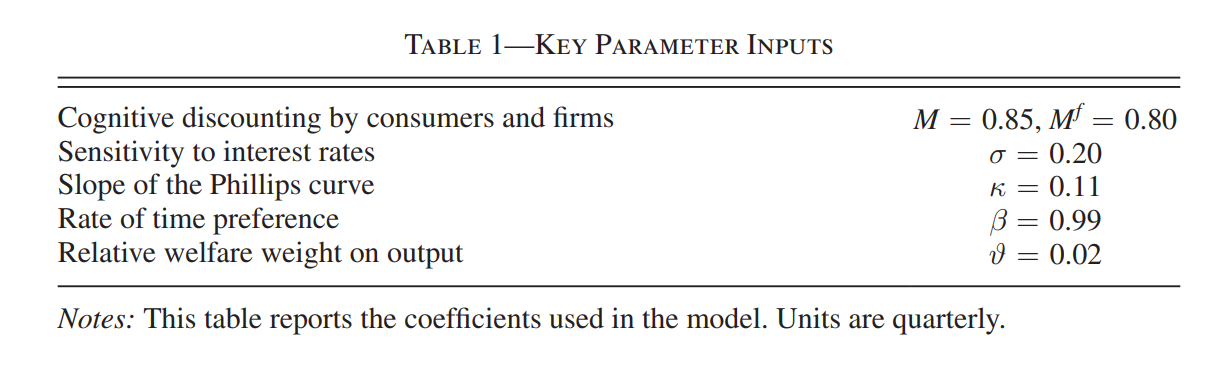
\includegraphics[width=\linewidth]{Table1.png}

\end{subfigure}
\begin{subfigure}{\textwidth}
  \centering
  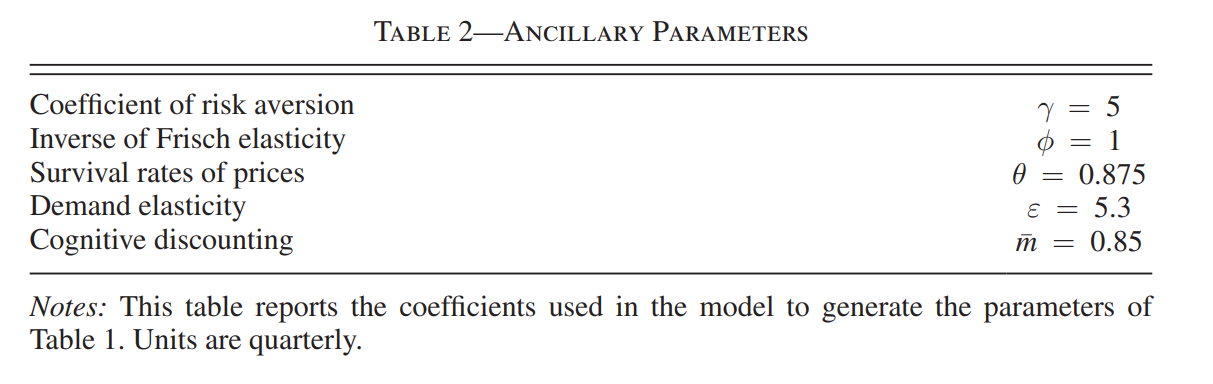
\includegraphics[width=\linewidth]{Table2.png}
 
\end{subfigure}
\end{figure}

\end{frame}

\section{Consequences}
\begin{frame}
    \ReduceFont
    \tableofcontents[currentsection, hideallsubsections]
\end{frame}

\begin{frame}
    \tableofcontents[currentsection, hideothersubsections, sections=\value{section}]
\end{frame}

\section{Implications for monetary policy}
\begin{frame}
    \ReduceFont
    \tableofcontents[currentsection, hideallsubsections]
\end{frame}

\begin{frame}
    \tableofcontents[currentsection, hideothersubsections, sections=\value{section}]
\end{frame}

\section{Implications for fiscal policy}
\begin{frame}
    \ReduceFont
    \tableofcontents[currentsection, hideallsubsections]
\end{frame}

\begin{frame}
    \tableofcontents[currentsection, hideothersubsections, sections=\value{section}]
\end{frame}

\section{Behavioral Enrichments of the Model}
\begin{frame}
    \ReduceFont
    \tableofcontents[currentsection, hideallsubsections]
\end{frame}

\begin{frame}
    \tableofcontents[currentsection, hideothersubsections, sections=\value{section}]
\end{frame}

\subsection{Term Structure of Consumer Attention}
\begin{frame}{\subsecname}
    \begin{equation} \tag{49}
        \begin{split}
            k_{t+1}= &\  \textbf{G}^{k,BR}(c_{t},N_{t},k_{t},\textbf{X}_{t}) \\
            & := (1+\bar{r}+\hat{r}^{BR}(\textbf{X}_t))(k_{t}+\bar{y}+\hat{y}^{BR}(N_{t},\textbf{X}_t)-c_{t})
        \end{split}
    \end{equation}
    \begin{equation}\tag{50}
        \begin{cases}
            \hat{r}^{BR} = m_{r} \hat{r}(\textbf{X}_{t}) \\
            \hat{y}^{BR}(N_{t},\textbf{X}_{t}) = m_{y}\hat{y}(\textbf{X}_{t})+\omega(\textbf{X}_{t})(N_{t}-N_{t}\textbf{X}_{t})
        \end{cases}
    \end{equation}
    \begin{equation}\tag{51}
        \begin{cases}
            \mathbb{E}_{t}^{BR}\left[\hat{r}^{BR}(\textbf{X}_{t+k})\right]=m_{r}\bar{m}^{k}\mathbb{E}_{t}\left[\hat{r}(\textbf{X}_{t+k})\right] \\
            \mathbb{E}_{t}^{BR}\left[\hat{y}^{BR}(\textbf{X}_{t+k})\right]=m_{r}\bar{m}^{k}\mathbb{E}_{t}\left[\hat{y}(\textbf{X}_{t+k})\right]
        \end{cases}
    \end{equation}
\end{frame}

\begin{frame}{\subsecname}
    \begin{equation}\tag{52}
        \hat{c}_{t}=\mathbb{E}_{t}\left[\sum_{\tau\geq t}\frac{\bar{m}^{\tau-t}}{R^{\tau-t}}\left(b_{r}m_{r}\hat{r}(\textbf{X}_{\tau})+m_{Y}\frac{\bar{r}}{R}\hat{y}(\textbf{X}_{\tau})\right)\right]
    \end{equation}
    \begin{equation}\tag{53}
        \frac{\Delta^{GE}}{\Delta^{\text{direct}}}=R^{\tau+1}
    \end{equation}
    \begin{equation}\tag{54}
        \frac{\Delta^{GE}}{\Delta^{\text{direct}}}=\left(\frac{R}{R-rm_{Y}}\right)^{\tau+1}\in\left[1, R^{\tau+1}\right]
    \end{equation}
\end{frame}


\subsection{Flattening of the Phillips Curve via Imperfect Firm Attention}
\begin{frame}{\subsecname}
    \begin{equation}\tag{55}
        \varv^{BR}(q_{it},(\textbf{X}_{\tau})):=\varv^{0}\left(q_{it}-m^{f}_{\pi}\Pi(\textbf{X}_{\tau}),m^{f}_{x}\mu(\textbf{X}_{\tau}),c(\textbf{X}_{\tau})\right)
    \end{equation}
    \begin{equation}\tag{56}
        \max_{q_{it}}{\mathbb{E}_{t}^{BR}\left[\sum_{\tau=t}^{\infty}\left(\beta\theta\right)^{\tau-t}\frac{c(\textbf{X}_{\tau})^{-\gamma}}{c(\textbf{X}_{\tau})^{-\gamma}}\varv^{BR}(q_{it},\textbf{X}_{\tau})\right]}
    \end{equation}
    \begin{equation}\tag{57}
        p^{*}_{t}=p_{t}+(1-\beta\theta)\sum^{\infty}_{k=0} \left(\beta\theta\bar{m}\right)^{k}\mathbb{E}_{t}\left[m^{f}_{\pi}(\pi_{t+1}+...+\pi_{t+k})-m^{f}_{x}\mu_{t+k}\right]
    \end{equation}
    \begin{equation}\tag{58}
        \kappa = m^{f}_{x}\bar{\kappa}
    \end{equation}
\end{frame}

\subsection{Nonconstant Trend Inflation and Neo- Fisherian Paradoxes}
\begin{frame}{\subsecname}
    \begin{equation}\tag{59}
        \pi^{d}_{t}=(1-\zeta)\bar{\pi}_{t}+\zeta\bar{\pi}_{t}^{CB}
    \end{equation}
    \begin{equation}\tag{60}
        x_{t}=M\mathbb{E}_{t}\left[x_{t+1}\right]-\sigma\left(i_{t}-\mathbb{E}_{t}\left[\pi_{t+1}\right]-r^{n}_{t}\right)
    \end{equation}
    \begin{equation}\tag{61}
        \pi_{t}=\beta\cdot M^{f} \mathbb{E}_t\left[\hat{\pi}_{t+1}\right]+\kappa\cdot x_{t}
    \end{equation}
    \begin{equation}\tag{62}
        \phi_{\pi}+\zeta \frac{(1-\beta M^{f})}{\kappa}\phi_{x}+\zeta\frac{(1-\beta M^{f})(1-M)}{\kappa \sigma}>1
    \end{equation}
\end{frame}

\section{Discussion of the Behavioral Assumptions, Conclusion, Critics}
\begin{frame}
    \ReduceFont
    \tableofcontents[currentsection, hideallsubsections]
\end{frame}

\begin{frame}
    \tableofcontents[currentsection, hideothersubsections, sections=\value{section}]
\end{frame}

\subsection{Behavioural enrichments}

\begin{frame}{\subsecname}
\textbf{Theoretical Microfoundations:} evidence exists for the inattention to small parameters, but no direct evidence on cognitive discounting. More empirical research on this is required despite the presence of extant evidence. Literature exists on cognitive discounting closely resembling hyperbolic discounting

\textbf{Lucas Critique:} Attention is endogenised in the appendix to reflect the fact that the attention becomes more intense when the volatility/deviation in the environment is more. Lucas critique hence becomes relevant for large changes. 

\end{frame}

\begin{frame}{\subsecname}
\textbf{Long Run Learning:} Learning and Attention is costly and require effort. Hence the agent might not learn anything in the long run. 

\textbf{Parsimony and new variants:} The current model is quite parsimonious and with just one standard parameter; $\bar{m}$. The term structure of attention enriches the model and the measurement of such an attention parameters is better. There is scope for improving the measurement of macro parameter of attention. Reasonable variations are possible for this model and the author chooses an \textit{"a happy balance between tractability, parsimony, and psychological and macroeconomic realism"}
\end{frame}

\subsection{Conclusion}
\begin{frame}{\subsecname}

1. This parsimonious model can be expanded examples include capital accumulation, a more frictional labor market, distortionary taxes, and agents that are heterogeneous in wealth or rationality.

2. Requirement for more empirical work to estimate attention to current variables and future variables.

3. Introduce survey designs which measures people's subjective view of the world. 

\end{frame}

\subsection{Critics}
\begin{frame}{\subsecname}

Overall the paper acknowledges that the model presented is parsimonious and more variations to it can be added. It more or less exhaustively covers the variations while discussing the possible behavioural enrichments. 

However, a few critiques \\
1. While modeling welfare for behavioral agents, the paper does not use subjective expectation. \\
2. It is possible that agents possess heterogeneous beliefs and can have different ways of expressing their partial myopia. \\
3. There is a need for more empirical testing for behavioral parameters, which the paper also acknowledges.


\end{frame}

\end{document}
